\documentclass[12pt, twoside]{article}
\usepackage[francais]{babel}
\usepackage[T1]{fontenc}
\usepackage[latin1]{inputenc}
\usepackage[left=7mm, right=1cm, top=1cm, bottom=7mm]{geometry}
\usepackage{float}
\usepackage{graphicx}
\usepackage{array}
\usepackage{multirow}
\usepackage{amsmath,amssymb,mathrsfs}
\usepackage{soul}
\usepackage{textcomp}
\usepackage{eurosym}
 \usepackage{variations}
\usepackage{tabvar}

\begin{document}


\section*{\center{Aide individualis�e: Triangles semblables}}

\subsection*{Rappels}
\begin{enumerate}
  \item Rappeler la d�finition de triangles semblables.
  
  \bigskip
  
  \bigskip
  

  
  \item Soit $ABC$ et $DEF$ deux triangles tels que $\widehat{A}=\widehat{D}$
  et $\widehat{B}=\widehat{E}$. Faire un sch�ma et le coder.
  
  \bigskip
  
  \bigskip
  
    \bigskip
  
  \bigskip  
  
  Que peut-on en d�duire? Justifier.
  
  \bigskip
  
  \bigskip
  
  \bigskip
  
  \item Compl�ter: Deux triangles sont de m�me forme (on dit aussi \ldots \ldots
  \ldots \ldots) si ils ont \ldots \ldots angles respectivement �gaux.
\end{enumerate}

\subsection*{Exercice 1}

Soit $A$, $B$ et $C$ trois points d'un cercle. la bissectrice de l'angle
$\widehat{ABC}$ coupe ce cercle en $D$ et $[AC]$ en $E$.

\begin{center}
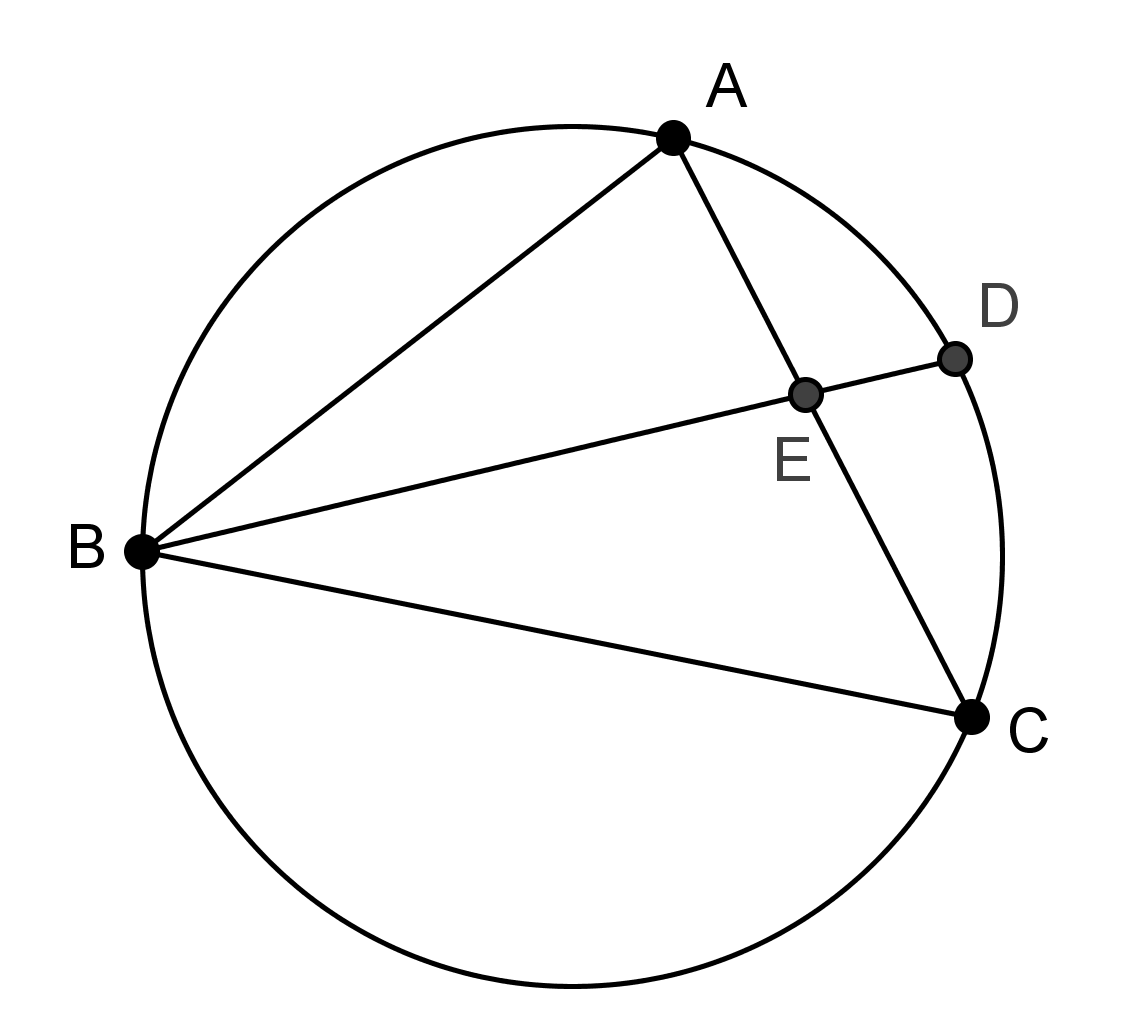
\includegraphics[width=5cm]{images/ex1.png}    
\end{center}

Le but est de montrer que les triangles $ABE$, $DCE$ et $DBC$ sont semblables.

\enskip

\begin{enumerate}
  \item  Sch�matiser les triangles $ABE$ et $BCD$
  
  \bigskip
  
  \bigskip
  
  \bigskip
  
  \bigskip
  
  \item Compl�ter:
  
  $(BD)$ est la bissectrice de \ldots \ldots donc $\widehat{ABD}=$\ldots \ldots.
  
  Or $\widehat{ABE}=\widehat{ABD}$ car \ldots \ldots \ldots \ldots \ldots
  \ldots \ldots
  
  Donc $\widehat{BDE}=$\ldots \ldots
  
  \medskip
  
 \textbf{ Coder cette information sur votre sch�ma et sur la figure initiale.}
  \item Compl�ter: $\widehat{BAC}=\widehat{BAE}$ car \ldots \ldots \ldots
  \ldots \ldots \ldots 
  
  $\widehat{BAC}$ et $\widehat{BDC}$ \ldots \ldots \ldots \ldots \ldots \ldots
  \ldots \ldots \ldots \ldots \ldots \ldots arc \ldots \ldots, donc \ldots
  \ldots
  \ldots
  
  d'o� $\widehat{BAE}=$\ldots \ldots
  
  \medskip
  
  \textbf{Coder cette information sur votre sch�ma et sur la figure initiale.}
  
  Que peut-on en d�duire sur les triangles $ABE$ et $BCD$?
  
  \bigskip
  
  \bigskip
  
  \item Sch�matiser les triangles $ABE$ et $EDC$.
  
  \bigskip
  
  \bigskip
  
  
  \item Comparer les angles $\widehat{AEB}$ et $\widehat{DEC}$.
  
  \bigskip
  
  \textbf{Coder cette information sur votre sch�ma et sur la figure initiale.}
  
  
  
  Que peut-on en d�duire sur les triangles $AEB$ et $DEC$?
  
  
\end{enumerate}


\subsection*{Exercice 2}

Les points $A$, $B$, $C$ et $D$ sont align�s tels que: $AB=BC=CD=4$. 

Le point
$S$ est tel que $SB=SC=SD=4$

\begin{center}
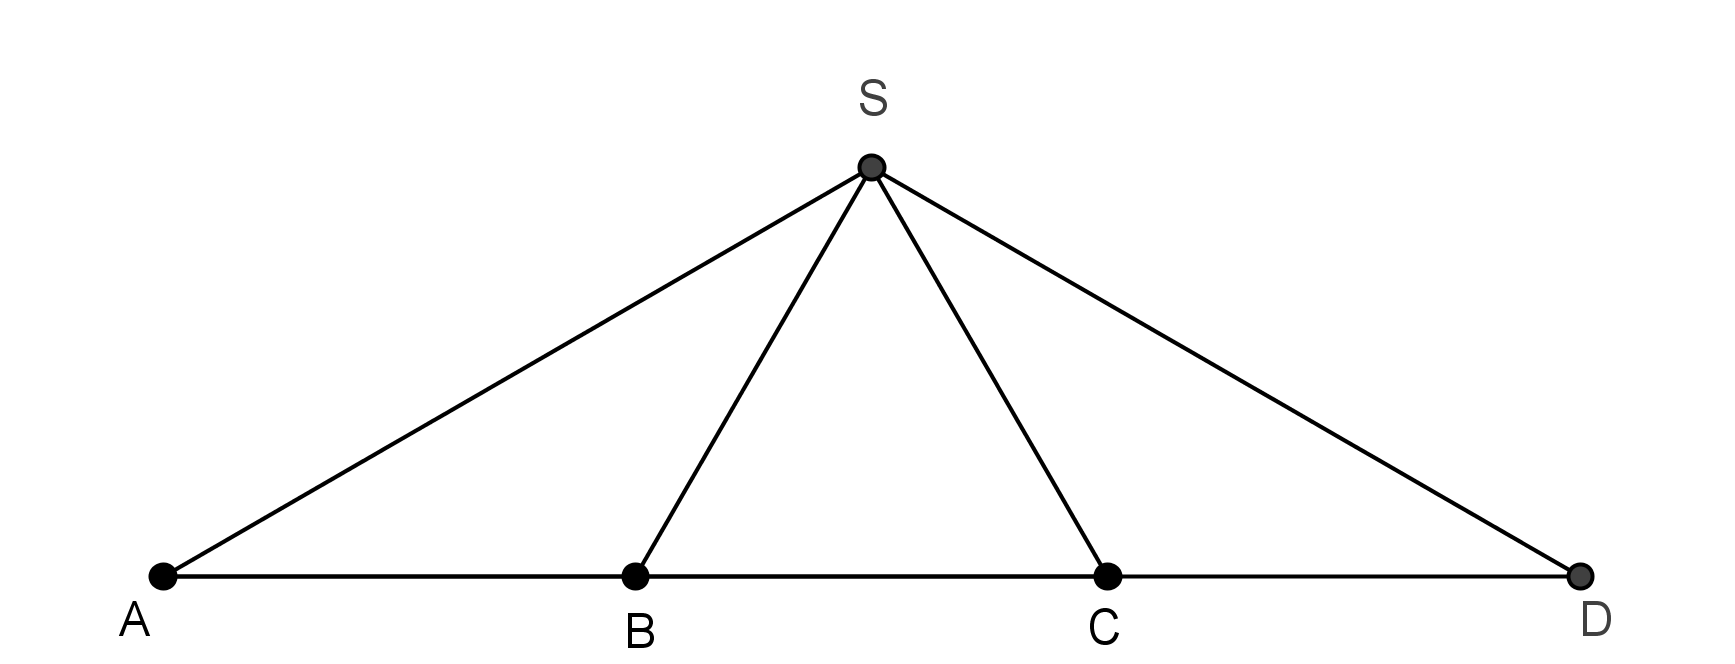
\includegraphics[width=9cm]{images/ex2.png}
\end{center}

\begin{enumerate}
  \item Coder la figure (et la coder au fur et � mesure que de nouvelles
  informations sont trouv�es).
  \item En d�duire les angles du triangle $SBC$.
  
\bigskip

\bigskip
  
  \item Que vaut l'angle $\widehat{SCD}$? En d�duire les angles du triangle
  $SCD$.
  
\bigskip

 \bigskip 
  
  \item Que peut-on dire des triangles $SAB$ et $SCD$? Justifier.
  
  \bigskip
  
  \bigskip
  
  \bigskip
  
  \bigskip
  
  \item Montrer que les triangles $SAD$ et $SCD$ sont semblables.
  
  \bigskip
  
  \bigskip
  
  \bigskip
  
  \bigskip
  
  \item Montrer que le triangle $SBD$ est rectangle en $S$. En d�duire $SD$.
  
  \bigskip
  
  \bigskip
  
  
  \bigskip
  
  \bigskip
  
  \bigskip
  
  \item Donner les sommets homologues. Calculer le rapport de proportionnalit�
  des c�t�s des triangles $DSA$ et $SCD$. En d�duire le rapport de leur aire.
\end{enumerate}

\end{document}
